\documentclass{article}\usepackage[]{graphicx}\usepackage[]{color}
%% maxwidth is the original width if it is less than linewidth
%% otherwise use linewidth (to make sure the graphics do not exceed the margin)
\makeatletter
\def\maxwidth{ %
  \ifdim\Gin@nat@width>\linewidth
    \linewidth
  \else
    \Gin@nat@width
  \fi
}
\makeatother

\definecolor{fgcolor}{rgb}{0.345, 0.345, 0.345}
\newcommand{\hlnum}[1]{\textcolor[rgb]{0.686,0.059,0.569}{#1}}%
\newcommand{\hlstr}[1]{\textcolor[rgb]{0.192,0.494,0.8}{#1}}%
\newcommand{\hlcom}[1]{\textcolor[rgb]{0.678,0.584,0.686}{\textit{#1}}}%
\newcommand{\hlopt}[1]{\textcolor[rgb]{0,0,0}{#1}}%
\newcommand{\hlstd}[1]{\textcolor[rgb]{0.345,0.345,0.345}{#1}}%
\newcommand{\hlkwa}[1]{\textcolor[rgb]{0.161,0.373,0.58}{\textbf{#1}}}%
\newcommand{\hlkwb}[1]{\textcolor[rgb]{0.69,0.353,0.396}{#1}}%
\newcommand{\hlkwc}[1]{\textcolor[rgb]{0.333,0.667,0.333}{#1}}%
\newcommand{\hlkwd}[1]{\textcolor[rgb]{0.737,0.353,0.396}{\textbf{#1}}}%
\let\hlipl\hlkwb

\usepackage{framed}
\makeatletter
\newenvironment{kframe}{%
 \def\at@end@of@kframe{}%
 \ifinner\ifhmode%
  \def\at@end@of@kframe{\end{minipage}}%
  \begin{minipage}{\columnwidth}%
 \fi\fi%
 \def\FrameCommand##1{\hskip\@totalleftmargin \hskip-\fboxsep
 \colorbox{shadecolor}{##1}\hskip-\fboxsep
     % There is no \\@totalrightmargin, so:
     \hskip-\linewidth \hskip-\@totalleftmargin \hskip\columnwidth}%
 \MakeFramed {\advance\hsize-\width
   \@totalleftmargin\z@ \linewidth\hsize
   \@setminipage}}%
 {\par\unskip\endMakeFramed%
 \at@end@of@kframe}
\makeatother

\definecolor{shadecolor}{rgb}{.97, .97, .97}
\definecolor{messagecolor}{rgb}{0, 0, 0}
\definecolor{warningcolor}{rgb}{1, 0, 1}
\definecolor{errorcolor}{rgb}{1, 0, 0}
\newenvironment{knitrout}{}{} % an empty environment to be redefined in TeX

\usepackage{alltt}

\usepackage{graphicx}
\usepackage[utf8]{inputenc}
\usepackage[T1]{fontenc}
\usepackage[english]{babel}
\usepackage{enumerate}
\usepackage{mathtools}
\usepackage{amsmath}
\usepackage{blindtext}
\usepackage{xspace}
\usepackage{hyperref}
\usepackage{amssymb}
\usepackage{url}
\usepackage{adjustbox}
%\usepackage{float}
%\usepackage{caption}
\usepackage{setspace}
\usepackage[margin=2.5cm]{geometry} 
\newgeometry{top=2.5cm, bottom=2.5cm}

\usepackage{apacite}
\bibliographystyle{apacite}


\title{A Bayesian Semiparametric Approach for Trend-Seasonal Interactions: an Application to Migration Forecasts. Additional Material}
\author{Alice Milivinti and Giacomo Benini}
\date{\today}
\IfFileExists{upquote.sty}{\usepackage{upquote}}{}
\begin{document}
\maketitle
\onehalfspacing






%%%%%%%%%%%%%%%%%%%%%%%%%%%%%%%%%%%%%%%%%%%%%%%%%%%%%%%%%
%%%%%%%%%%%%%%%%%%%%%%%%%%%%%%%%%%%%%%%%%%%%%%%%%%%%%%%%%
\section{Bayesian Analysis}\label{bayesian analysis}
%%%%%%%%%%%%%%%%%%%%%%%%%%%%%%%%%%%%%%%%%%%%%%%%%%%%%%%%%
%%%%%%%%%%%%%%%%%%%%%%%%%%%%%%%%%%%%%%%%%%%%%%%%%%%%%%%%%

In this section we provide an overview of the Bayesian method on which our forecasts are based on. We illustrate how Bayesian techniques are implemented starting by rewriting equation (6) of the 1st order Fourier in matrix form 
\begin{align}\label{matrix_bayes}
\mathbf{y}_{t}&= \mathbf{\varphi} \mathbf{x}_{t}+\epsilon_{t} \quad \quad \epsilon_{t} \sim N(0, \sigma_{\epsilon}^{2}), 
\end{align}  
where $ \mathbf{\varphi}=[\beta_{0}, \beta_{1}, \beta_{21}, \beta_{31}]^{T}$ and  $ \mathbf{x}_{t}=[1, \text{trend}_{t}, \cos_{1t}+\sin_{1t}, \text{trend}_{t}*(\cos_{1t}+\sin_{1t})] $.
\begin{description}

\item[STEP I] Assume a prior probability distribution for $\mathbf{\varphi} \sim  P(\mathbf{\varphi | \alpha})$, where $\mathbf{\alpha}$ are the parameters, which identify the prior distribution, i.e. the hyperparameter. The prior is the probability of $\mathbf{\varphi}$ which reflects the researcher's expectations.

\item[STEP II] Use the collected data $\mathbf{x}_{t}$ to compute the likelihood of the sample,
\begin{align}\label{likelihood}
P(\mathbf{x_t | \mathbf{\varphi}}) = \prod_{t=1}^{T}g(\mathbf{x}_t| \mathbf{\varphi}),
\end{align}
where $ g(\cdot) $ is the probability density function of the data.

\item[STEP III] According to the Bayes' rule, update the prior beliefs using the information contained in the likelihood obtaining the posterior distribution

\begin{align}\label{posteriorr}
P(\mathbf{\varphi | x_t, \alpha}) = \frac{P(\mathbf{x_t | \varphi}) P(\mathbf{\varphi | \alpha})}{P(\mathbf{x_t | \alpha})}
\end{align}

that is, the probability of observing the hypothesis $\mathbf{\alpha}$ given the observed data $\mathbf{x_t} $.
Given the difficulty to accurately compute the marginal likelihood $ P(\mathbf{x_t | \alpha})$, the posterior is often approximated by $ P(\mathbf{\varphi | x_t, \alpha}) \propto P(\mathbf{x_t | \varphi}) P(\mathbf{\varphi | \alpha}) $.
\end{description}
The formalization of the Bayesian method shows how this methodology embodies the forecast principles combining probabilistic statements about the model's parameters $ \mathbf{\varphi} $ and the available data $ (\mathbf{y}_t,\mathbf{x}_t) $ \shortcite{geweke2006bayesian}. The resulting predictive probability is obtained by integrating over the posterior distribution,
\begin{align}\label{int}
G(\mathbf{\hat{y}_t} | \mathbf{x_t, \alpha}) = \int_{\mathbf{\varphi}} P(\mathbf{y_t} | \mathbf{\varphi}) P(\mathbf{\varphi} | \mathbf{x_t}, \mathbf{\alpha}) \text{d}\mathbf{\varphi}.
\end{align}
To compute such integrations, analytical solutions are generally hard to find and therefore numerical approximations are used. The procedure just described is able to produce accurate forecasts for parametric models. However, it cannot be implemented for the semiparametric specifications. The next section illustrates how to adapt these three steps to equations where at least one of the arguments is a nonparametric function. 

%%%%%%%%%%%%%%%%%%%%%%%%%%%%%%%%%%%%%%%%%%%%%%%%%%%%%%%%%%%%%%%%%%%%%%%%%%%%%%%%%%%%
%%%%%%%%%%%%%%%%%%%%%%%%%%%%%%%%%%%%%%%%%%%%%%%%%%%%%%%%%%%%%%%%%%%%%%%%%%%%%%%%%%%%
\subsection{Nonparametric Bayesian Techniques} \label{nonparametric techniques}
%%%%%%%%%%%%%%%%%%%%%%%%%%%%%%%%%%%%%%%%%%%%%%%%%%%%%%%%%%%%%%%%%%%%%%%%%%%%%%%%%%%%
%%%%%%%%%%%%%%%%%%%%%%%%%%%%%%%%%%%%%%%%%%%%%%%%%%%%%%%%%%%%%%%%%%%%%%%%%%%%%%%%%%%%

Unlike equation (\ref{matrix_bayes}), the semiparametric specifications require a prior distribution on a function. This reflects the need to make an assumption about every point in some continuous input space to which associate a certain statistical process. One of the most common choices is to assume that all the arguments are normally distributed random variables, so that the functions $ f_1(\cdot), f_{21} (\cdot), f_{31}(\cdot)$ follow a Gaussian Process (GP),
\begin{align}\label{GP}
f_1(\cdot) \sim GP(\cdot | 0, \sigma_{f_1}^2) \quad f_{21}(\cdot) \sim GP(\cdot | 0, \sigma_{f_{21}}^2) \quad f_{31}(\cdot) \sim GP(\cdot | 0, \sigma_{f_{31}}^2).
\end{align}
The practical application of this relatively straightforward generalization of \textbf{STEP I} is rather convoluted and depends crucially upon the way the $ f(\cdot) $s are computed. Therefore, before seeing how (\ref{GP}) allows to replicate the procedure illustrated in the previous section, it is necessary to decide how to estimate $ \hat{f}_1(\cdot), \hat{f}_{21}(\cdot),  \hat{f}_{31}(\cdot)$. Among the different options available to fit unknown functions, thin plate regression splines deliver the most efficient smoothers \cite{wood2003thin}. Therefore, we use them to construct composite curves for which the last point of the first curve coincides with the first point of the second curve such that these two points have the same tangent (first derivative) and curvature (second derivative). Given the aim to re-adapt \textbf{STEP I} to the "prior assumption" (\ref{GP}), we re-write equation 
\begin{align}\label{fourier_gam_int_1st}
y_{t}=\beta_{0}+f_{1}(\text{trend}_{t})+f_{21}(\cos_{1t}+\sin_{1t})+f_{31}(\text{trend}_{t}, \cos_{1t}+\sin_{1t})+\epsilon_{t},
\end{align}
in matrix form,
\begin{align}\label{GAM}
\mathbf{y}_t= h(\mathbf{p}_t) + \epsilon_t. 
\end{align}
Thin-plate regression splines can be estimated minimizing for $\mathbf{h}$
\begin{align}\label{euclidian}
|| \mathbf{y} - \mathbf{h} ||^{2} + \lambda J_{md}(h),
\end{align}
where $ \mathbf{y} $ is a vector containing the data points $ [y_{1}, y_{2}, ..., y_{T}] $, $ \mathbf{h} = [f_{1}(\mathbf{p}_1), f_{21}(\mathbf{p}_2), f_{31}(\mathbf{p}_3)]$, with $ \mathbf{p}_1 = [\text{trend}_{t}] $, $ \mathbf{p}_2 = [\cos_{1t}+\sin_{1t}] $ and $ \mathbf{p}_3 = [\text{trend}_{t}, \cos_{1t}+\sin_{1t}] $, $ \lambda $ is a smoothing parameter and $ J_{md}(h) $ is a penalty function which measures the wiggliness of $h$. The particular form taken by $ J_{md}(h) $ is   
\begin{align} \label{penalty}
J_{md} = \int ... \int_{\Re^d} \sum_{\nu_1+...\nu_d = m} \frac{m!}{\nu_1!...\nu_d!} \Big( \frac{\partial^m h}{\partial p_1^{\nu_1}...\partial p_d^{\nu_d}} \Big)^2 d p_1...d p_d ,
\end{align}
where $T+1$ is a sequence of non-decreasing real numbers which define the domain of each basis function \cite{duchon1977splines}. 

Minimization (\ref{euclidian}) includes the smoothing parameter $\lambda \in [0,\infty )$ which controls for the trade-off between model fit and smoothness. If $\lambda \rightarrow \infty$, $\hat{h}$ is a straight line estimate converging to the linear least squares estimate. If $\lambda \rightarrow 0$, $\hat{h}$ is an un-penalized regression spline estimate  suffering from an over-fitting issue \cite{de1978practical}. Solving (\ref{euclidian}), for a fixed $\lambda $, allows to write the estimate of $h$ as a thin plate regression splne, 
\begin{align}
\hat{h}_{\lambda }(\mathbf{p}) = \sum _{j=1}^ M \theta_j \phi_j(\mathbf{p})+ \sum_t^T \delta_t \eta_{md}(\| \mathbf{p}-\mathbf{p}_t \| ) ,
\end{align}
where $\delta_t$ and $\theta_j$ are coefficients to be estimated and $\phi_j(\mathbf{p})$ is the vector of $M={m+d-1\choose d}$ unpenalized polynomials of $\mathbf{p}$ with degrees up to $m-1$. Beside $\phi_j(\mathbf{p})$, $\eta_{m,d}$, which is a function of the Euclidean distance $r$ between any $\mathbf{p}$ and the observed $\mathbf{p}_t$ values, models the additional non-linearity:
\begin{align} 
\eta _{m,d}(r) = \begin{cases} \frac{(-1)^{m+1+d/2}}{2^{2m-1}\pi ^{d/2}(m-1)!(m-d/2)!}r^{2m-d}\log (r) & \text {if } d \text { even}\\ \frac{\Gamma (d/2-m)}{2^{2m}\pi ^{d/2}(m-1)!}r^{2m-d} & \text {if } d \text { odd.} \end{cases}
\end{align}
By defining the penalty matrix $\mathbf{E}$ such that each entry $e_{tj}\equiv \eta _{m,d}(\| \mathbf{p}_t -\mathbf{p}_ j\| )$, the function estimate $\hat{h}_{\lambda }$ is then obtained by minimizing equation (\ref{minimization2}) with respect to $ \delta$ and $\theta$ :
\begin{align} \label{minimization2}
\min \| \mathbf{\mathbf{y}-C \theta -E \delta} \| ^2+\lambda \mathbf {\delta' E \delta}, \quad \mathbf {C' \delta } =\mathbf{0},
\end{align}
where, $\mathbf{y}$ is the responses' vector, $\mathbf{C}$ is the matrix whose rows are $\phi_j(\mathbf{p})$, $\mathbf{\theta}$ and $\mathbf{\delta}$ are vectors of coefficients $\theta_j$ and $\delta_t$ \cite{wood2006generalized}. Besides the great flexibility qualities of the thin plate regression spline as a smoother, the estimate of $\hat{h}_{\lambda}$ engages as many parameters as the number of data points, generating important computational costs. Therefore, solving $(\mathbf{\theta ,\delta} )$ with an optimum $\lambda^*$ becomes difficult for large problems. Being $\mathbf{E} $ a symmetric and non-negative definite matrix, the eigen-decomposition can be written as $\mathbf{E = U D U'}$, where $\mathbf{D} $ is the diagonal matrix of $d_{t}$ eigenvalues of $\mathbf{E} $ and $\mathbf{U}$ is the corresponding eigenvectors matrix. The truncated eigen-decomposition produces $\tilde{\mathbf{E}}_ k$, which is an approximation to $\mathbf{E} $ such that
\[ \tilde{\mathbf{E }}_k = \mathbf{U}_k \mathbf{D}_k \mathbf{U}_k' \]
where $\mathbf{D}_k$ is a diagonal matrix that contains the $k$ most extreme eigenvalues in descending order of absolute values (i.e. the top right $k \times k$ sub-matrix of $\mathbf{D}$): $|\tilde{d}_1|>\cdots >|\tilde{d}_ k|$. $\mathbf{U}_k$ is the eigenvectors matrix corresponding to the eigenvalues in $\mathbf{D}_k$. The approximation $\tilde{\mathbf{E}}_k$ brings some advantages. First it reduces the dimension from $T\times T$ of $\mathbf{E}$ to $T\times k$. Second, $\tilde{\mathbf{E}}_k$ minimizes the spectral norm $\| \mathbf{E} -\mathbf{F}_k\| _2$ between $\mathbf{E}$ and all rank $k$ matrices $\mathbf{F}_k$. Third, $\tilde{\mathbf{E}}_k$ minimizes the worst possible change in the shape of the spline introduced by the eigen-space truncation measured by

\[ \max_{\mathbf{\delta} \ne 0} \frac{\mathbf{\delta} '(\mathbf{E} - \mathbf{G}_k) \delta}{\| \mathbf{\delta} \| ^2}, \]
where $\mathbf{G}_k$ is formed by any $k$ eigenvalues and corresponding eigenvectors \cite{wood2003thin}. Given $\mathbf{E} \approx \tilde{\mathbf{E}}_k$ and $\tilde{\mathbf{E}}_k = \mathbf{U}_k \mathbf{D}_k \mathbf{U}_k'$ and letting $\mathbf{\delta}_k= \mathbf{U}_k' \mathbf{\delta}$, the minimization problem becomes
\begin{align*}
\min \| \mathbf{\mathbf{y} -C \theta} - \mathbf{U}_k \mathbf{D}_k \mathbf{\delta}_k \|^2 + \mathbf{\lambda \delta}_k' \mathbf{D}_k \mathbf{\delta}_k \quad \text{subject to} \quad \mathbf{C' U}_k \mathbf{\delta}_k= 0. 
\end{align*}
The constrained optimization problem can be converted into an unconstrained one by using any orthogonal column basis $\mathbf{Z} $. One way to form $\mathbf{Z} $ is via the QR decomposition of $\mathbf{U}_k' \mathbf{C} $:
\[ \mathbf{U}_k' \mathbf{C} = [\mathbf{Q_1 Q_2}] \left[\begin{matrix} \mathbf{R} \\ \mathbf{0} \end{matrix}\right]. \]
Letting $\mathbf{Z = Q_2}$, it is verified that
\[ \mathbf{T' U}_k \mathbf{Z = R' Q_1' Q_2 = 0.} \]
Therefore, it is true that $\mathbf{\delta}_k= \mathbf{Z \tilde{\delta}}$ for $\mathbf{\delta}_k$ such that $\mathbf{C' U}_k \mathbf{\delta}_k = 0$. Now the problem becomes the unconstrained optimization,
\begin{align*}
\min \| \mathbf{\mathbf{y} -C \theta} - \mathbf{U}_k \mathbf{D}_k \mathbf{Z \tilde{\delta}}\|^2+ \lambda \mathbf{\tilde{\delta}' Z'} \mathbf{D}_k \mathbf{Z \tilde{\delta}}.
\end{align*}
By defining
\[ \mathbf{\kappa} = \left[\begin{matrix} \mathbf{\theta} \\ \mathbf{\tilde{\delta}} \end{matrix}\right], \quad \mathbf{\mathbf{p}} = [\mathbf{C : U}_k \mathbf{D}_k \mathbf{Z}], \quad \text {and} \quad \mathbf{S} = \left[\begin{matrix} \mathbf{0} & \mathbf{0} \\ \mathbf{0} & \mathbf{Z' D}_k \mathbf{Z} \end{matrix}\right] \]
the optimization can be simplified as $ \min \| \mathbf{y - p \kappa} \| ^2 + \lambda \mathbf{\kappa' S \kappa} $ with respect to $\mathbf{\kappa}$. This last reformulation of the minimization problem allows to rethink (\ref{GP}) in terms of assumptions about the distribution of $ \mathbf{\lambda} $ and of $ \mathbf{\kappa} $. In particular, if 
\begin{align}\label{GP_1}
f_1(\cdot) \sim GP(\cdot | 0, 1) \quad f_{21}(\cdot) \sim GP(\cdot | 0, 1) \quad f_{31}(\cdot) \sim GP(\cdot | 0, 1),
\end{align}
then it is possible to assume as priors $ \kappa \sim N(0,1) $ and $ \lambda \sim N(0,\sigma_{\lambda}^{2}) $ and start the estimation process.

\section{Simulations Results}\label{simumations}

This section provides the simulations' codes as well as the results' visualization of the fitting and forecasts of the linear, the semi- and the non- parametric models with and without interaction (see section 2.2 of the paper).

\begin{knitrout}
\definecolor{shadecolor}{rgb}{0.969, 0.969, 0.969}\color{fgcolor}\begin{kframe}
\begin{alltt}
\hlstd{freq} \hlkwb{<-} \hlnum{12}
\hlstd{years} \hlkwb{<-} \hlnum{30}
\hlstd{N} \hlkwb{<-} \hlstd{freq}\hlopt{*}\hlstd{years}
\hlstd{x} \hlkwb{<-} \hlstd{(}\hlnum{1}\hlopt{:}\hlstd{N)}\hlopt{/}\hlstd{freq}

\hlkwd{set.seed}\hlstd{(}\hlnum{1}\hlstd{)}

\hlcom{##########################################################################}
\hlcom{# SIMULATION 1.1: 1st order Fourier trend, seasonality no interaction}
\hlcom{##########################################################################}

\hlcom{# Trend}
\hlstd{trend_11} \hlkwb{<-} \hlkwd{cumsum}\hlstd{(}\hlkwd{cumsum}\hlstd{(}\hlkwd{rnorm}\hlstd{(N))}\hlopt{+}\hlkwd{rnorm}\hlstd{(N))}

\hlcom{# Seasonality}
\hlstd{sea_11} \hlkwb{<-} \hlnum{.3} \hlopt{+} \hlnum{3}\hlopt{*}\hlkwd{cos}\hlstd{(}\hlnum{2}\hlopt{*}\hlstd{pi}\hlopt{*}\hlstd{x)} \hlopt{+} \hlnum{6}\hlopt{*}\hlkwd{sin}\hlstd{(}\hlnum{2}\hlopt{*}\hlstd{pi}\hlopt{*}\hlstd{x)}

\hlcom{# Time Series data}
\hlstd{sim_11} \hlkwb{<-} \hlkwd{as.data.frame}\hlstd{(}\hlkwd{abs}\hlstd{(}\hlnum{0.4}\hlopt{*}\hlstd{trend_11} \hlopt{+} \hlnum{10}\hlopt{*}\hlstd{sea_11} \hlopt{+} \hlnum{.2}\hlopt{*}\hlkwd{rnorm}\hlstd{(N)))}

\hlcom{##########################################################################}
\hlcom{# SIMULATION 2.1: 2nd order Fourier trend, seasonality no interaction}
\hlcom{##########################################################################}
\hlkwd{set.seed}\hlstd{(}\hlnum{1}\hlstd{)}
\hlcom{# Trend}
\hlstd{trend_21} \hlkwb{<-} \hlkwd{cumsum}\hlstd{(}\hlkwd{cumsum}\hlstd{(}\hlkwd{rnorm}\hlstd{(N))}\hlopt{+}\hlkwd{rnorm}\hlstd{(N))}

\hlcom{# Seasonality}
\hlstd{sea_21} \hlkwb{<-} \hlnum{.3} \hlopt{+} \hlnum{.5}\hlopt{*}\hlkwd{cos}\hlstd{(}\hlnum{2}\hlopt{*}\hlstd{pi}\hlopt{*}\hlstd{x)} \hlopt{+} \hlnum{1.2}\hlopt{*}\hlkwd{sin}\hlstd{(}\hlnum{2}\hlopt{*}\hlstd{pi}\hlopt{*}\hlstd{x)} \hlopt{+}
  \hlnum{.6}\hlopt{*}\hlkwd{cos}\hlstd{(}\hlnum{2}\hlopt{*}\hlnum{2}\hlopt{*}\hlstd{pi}\hlopt{*}\hlstd{x)} \hlopt{+} \hlnum{.2}\hlopt{*}\hlkwd{sin}\hlstd{(}\hlnum{2}\hlopt{*}\hlnum{2}\hlopt{*}\hlstd{pi}\hlopt{*}\hlstd{x)}

\hlcom{# Time Series data}
\hlstd{sim_21} \hlkwb{<-} \hlkwd{as.data.frame}\hlstd{(}\hlkwd{abs}\hlstd{(}\hlnum{0.1}\hlopt{*}\hlstd{trend_21} \hlopt{+} \hlnum{40}\hlopt{*}\hlstd{sea_21} \hlopt{+} \hlnum{.2}\hlopt{*}\hlkwd{rnorm}\hlstd{(N)))}


\hlcom{##########################################################################}
\hlcom{# SIMULATION 1.2: 1st order Fourier trend, seasonality with interaction}
\hlcom{##########################################################################}
\hlkwd{set.seed}\hlstd{(}\hlnum{1}\hlstd{)}

\hlcom{# Trend}
\hlstd{trend_12} \hlkwb{<-} \hlkwd{cumsum}\hlstd{(}\hlkwd{cumsum}\hlstd{(}\hlkwd{rnorm}\hlstd{(N))}\hlopt{+}\hlkwd{rnorm}\hlstd{(N))}

\hlcom{# Seasonality}
\hlstd{sea_12} \hlkwb{<-} \hlnum{.3} \hlopt{+} \hlnum{3}\hlopt{*}\hlkwd{cos}\hlstd{(}\hlnum{2}\hlopt{*}\hlstd{pi}\hlopt{*}\hlstd{x)} \hlopt{+} \hlnum{6}\hlopt{*}\hlkwd{sin}\hlstd{(}\hlnum{2}\hlopt{*}\hlstd{pi}\hlopt{*}\hlstd{x)}

\hlcom{# Time Series data}
\hlstd{sim_12} \hlkwb{<-} \hlkwd{as.data.frame}\hlstd{(}\hlnum{0.4}\hlopt{*}\hlstd{trend_12} \hlopt{+} \hlnum{24}\hlopt{*}\hlstd{sea_12} \hlopt{+} \hlnum{0.8}\hlopt{*}\hlstd{trend_12}\hlopt{*}\hlstd{sea_12} \hlopt{+} \hlnum{.2}\hlopt{*}\hlkwd{rnorm}\hlstd{(N))}


\hlcom{##########################################################################}
\hlcom{# SIMULATION 2.2: 2nd order Fourier trend, seasonality with interaction}
\hlcom{##########################################################################}

\hlkwd{set.seed}\hlstd{(}\hlnum{1}\hlstd{)}
\hlcom{# Trend}
\hlstd{trend_22} \hlkwb{<-} \hlkwd{cumsum}\hlstd{(}\hlkwd{cumsum}\hlstd{(}\hlkwd{rnorm}\hlstd{(N))}\hlopt{+}\hlkwd{rnorm}\hlstd{(N))}
\hlcom{# Seasonality}
\hlstd{sea_22} \hlkwb{<-} \hlnum{.3} \hlopt{+} \hlnum{.5}\hlopt{*}\hlkwd{cos}\hlstd{(}\hlnum{2}\hlopt{*}\hlstd{pi}\hlopt{*}\hlstd{x)} \hlopt{+} \hlnum{1.2}\hlopt{*}\hlkwd{sin}\hlstd{(}\hlnum{2}\hlopt{*}\hlstd{pi}\hlopt{*}\hlstd{x)} \hlopt{+}
  \hlnum{.6}\hlopt{*}\hlkwd{cos}\hlstd{(}\hlnum{2}\hlopt{*}\hlnum{2}\hlopt{*}\hlstd{pi}\hlopt{*}\hlstd{x)} \hlopt{+} \hlnum{.2}\hlopt{*}\hlkwd{sin}\hlstd{(}\hlnum{2}\hlopt{*}\hlnum{2}\hlopt{*}\hlstd{pi}\hlopt{*}\hlstd{x)}

\hlcom{# Time Series data}
\hlstd{sim_22} \hlkwb{<-} \hlkwd{as.data.frame}\hlstd{(}\hlnum{0.4}\hlopt{*}\hlstd{trend_22} \hlopt{+} \hlnum{24}\hlopt{*}\hlstd{sea_22} \hlopt{+} \hlnum{0.8}\hlopt{*}\hlstd{trend_22}\hlopt{*}\hlstd{sea_22} \hlopt{+} \hlnum{.2}\hlopt{*}\hlkwd{rnorm}\hlstd{(N))}

\hlcom{###################################################################################}
\hlcom{# SIMULATION 1.3: 1st order Fourier trend, seasonality with complex interaction}
\hlcom{###################################################################################}
\hlkwd{set.seed}\hlstd{(}\hlnum{1}\hlstd{)}

\hlcom{# Trend}
\hlstd{trend_13} \hlkwb{<-} \hlkwd{sqrt}\hlstd{(}\hlkwd{cumsum}\hlstd{(}\hlkwd{cumsum}\hlstd{(}\hlkwd{rnorm}\hlstd{(N)))}\hlopt{+}\hlkwd{rnorm}\hlstd{(N))}

\hlcom{# Seasonality}
\hlstd{sea_13} \hlkwb{<-} \hlnum{.3} \hlopt{+} \hlnum{3}\hlopt{*}\hlkwd{cos}\hlstd{(}\hlnum{2}\hlopt{*}\hlstd{pi}\hlopt{*}\hlstd{x)} \hlopt{+} \hlnum{6}\hlopt{*}\hlkwd{sin}\hlstd{(}\hlnum{2}\hlopt{*}\hlstd{pi}\hlopt{*}\hlstd{x)}

\hlcom{# Time Series data}
\hlstd{sim_13} \hlkwb{<-} \hlkwd{as.data.frame}\hlstd{(}\hlnum{3} \hlopt{+} \hlnum{15}\hlopt{*}\hlstd{trend_13} \hlopt{+} \hlnum{10}\hlopt{*}\hlkwd{exp}\hlstd{(sea_13)}\hlopt{*}\hlstd{trend_13} \hlopt{+} \hlnum{.4}\hlopt{*}\hlkwd{rnorm}\hlstd{(N))}



\hlcom{###################################################################################}
\hlcom{# SIMULATION 2.3: 2nd order Fourier trend, seasonality with complex interaction}
\hlcom{###################################################################################}
\hlkwd{set.seed}\hlstd{(}\hlnum{1}\hlstd{)}
\hlcom{# Trend}
\hlstd{trend_23} \hlkwb{<-} \hlkwd{sqrt}\hlstd{(}\hlkwd{cumsum}\hlstd{(}\hlkwd{cumsum}\hlstd{(}\hlkwd{rnorm}\hlstd{(N)))}\hlopt{+}\hlkwd{rnorm}\hlstd{(N))}

\hlcom{# Seasonality}
\hlstd{sea_23} \hlkwb{<-} \hlnum{.3} \hlopt{+} \hlnum{.5}\hlopt{*}\hlkwd{cos}\hlstd{(}\hlnum{2}\hlopt{*}\hlstd{pi}\hlopt{*}\hlstd{x)} \hlopt{+} \hlnum{1.2}\hlopt{*}\hlkwd{sin}\hlstd{(}\hlnum{2}\hlopt{*}\hlstd{pi}\hlopt{*}\hlstd{x)} \hlopt{+}
  \hlnum{.6}\hlopt{*}\hlkwd{cos}\hlstd{(}\hlnum{2}\hlopt{*}\hlnum{2}\hlopt{*}\hlstd{pi}\hlopt{*}\hlstd{x)} \hlopt{+} \hlnum{.2}\hlopt{*}\hlkwd{sin}\hlstd{(}\hlnum{2}\hlopt{*}\hlnum{2}\hlopt{*}\hlstd{pi}\hlopt{*}\hlstd{x)}

\hlcom{# Time Series data}
\hlstd{sim_23} \hlkwb{<-} \hlkwd{as.data.frame}\hlstd{(}\hlnum{3} \hlopt{+} \hlnum{15}\hlopt{*}\hlstd{trend_23} \hlopt{+} \hlnum{10}\hlopt{*}\hlkwd{exp}\hlstd{(sea_23)}\hlopt{*}\hlstd{trend_23} \hlopt{+} \hlnum{.4}\hlopt{*}\hlkwd{rnorm}\hlstd{(N))}
\end{alltt}
\end{kframe}
\end{knitrout}

\begin{figure}[bp!]
\centering
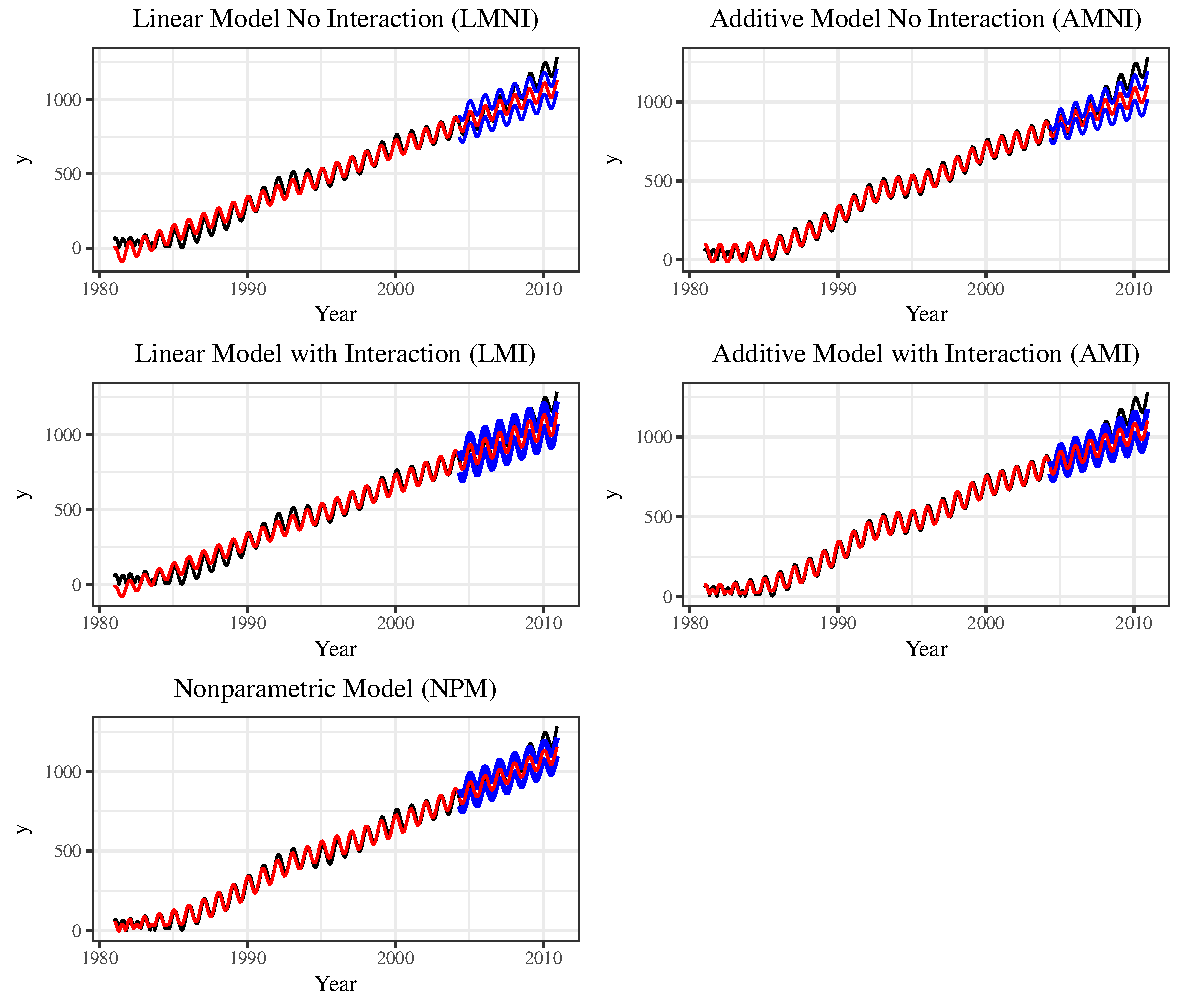
\includegraphics[scale=0.7]{1st_order_no_inter.pdf}
\caption{1st order Fourier series with no interaction: fitting and forecasts results for different models.}
\label{fig:1st Fourier no inter}
\end{figure}


\begin{figure}[bp!]
\centering
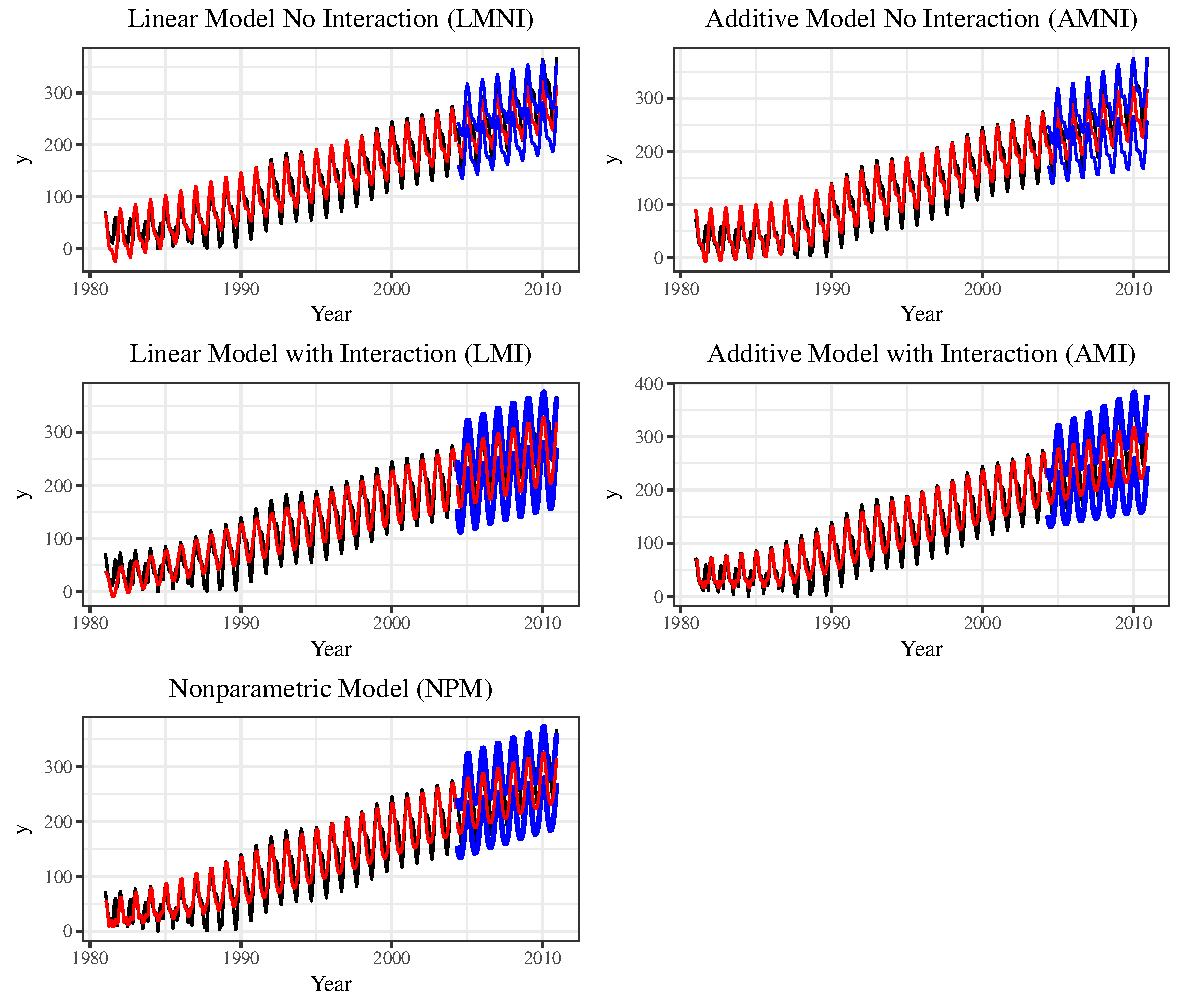
\includegraphics[scale=0.7]{2nd_order_no_inter.pdf}
\caption{2nd order Fourier series with no interaction: fitting and forecasts results for different models.}
\label{fig:2nd Fourier no inter}
\end{figure}

\begin{figure}[bp!]
\centering
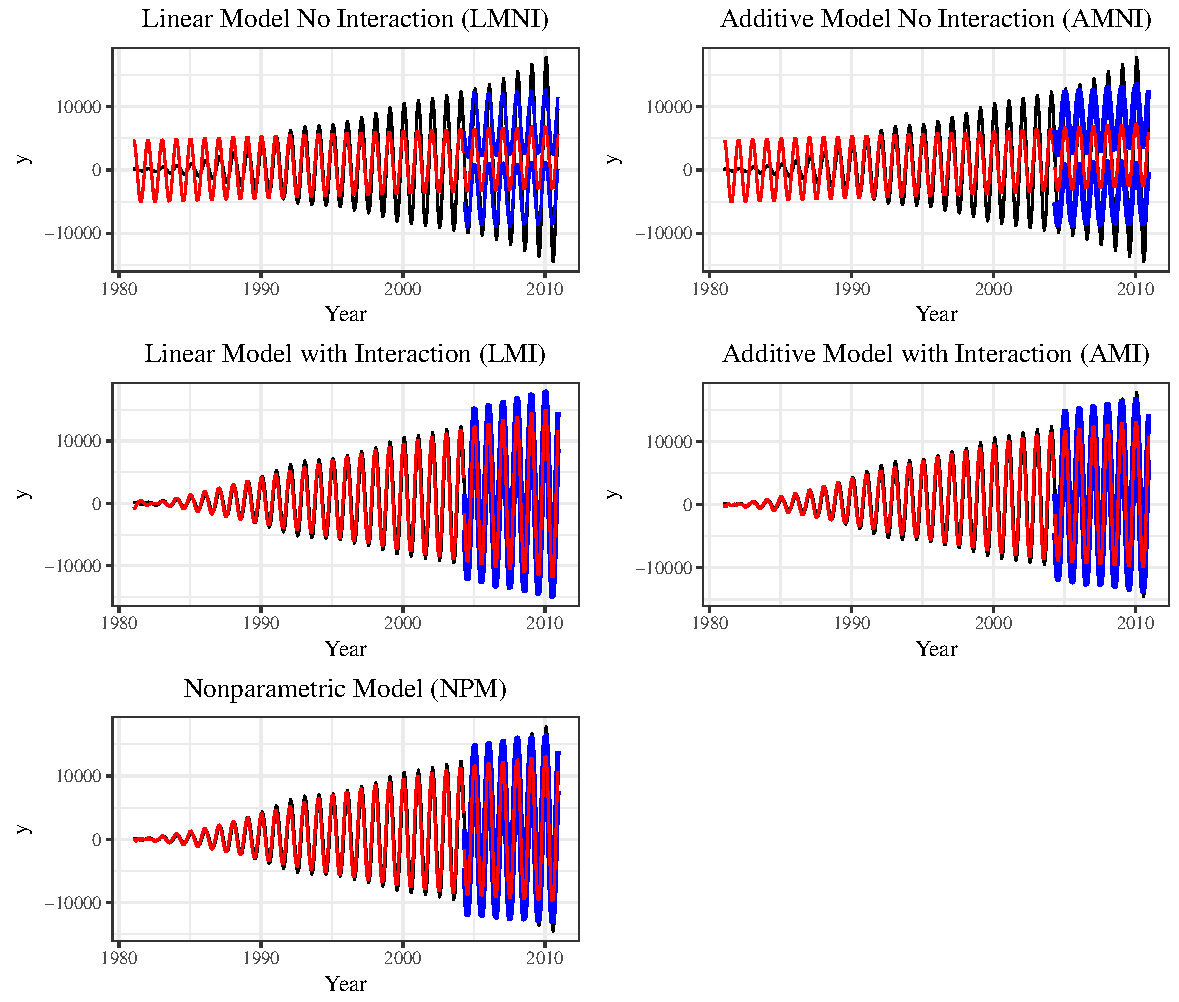
\includegraphics[scale=0.7]{1st_order_inter.pdf}
\caption{1st order Fourier series with interaction: fitting and forecasts results for different models.}
\label{fig:1st Fourier inter}
\end{figure}


\begin{figure}[bp!]
\centering
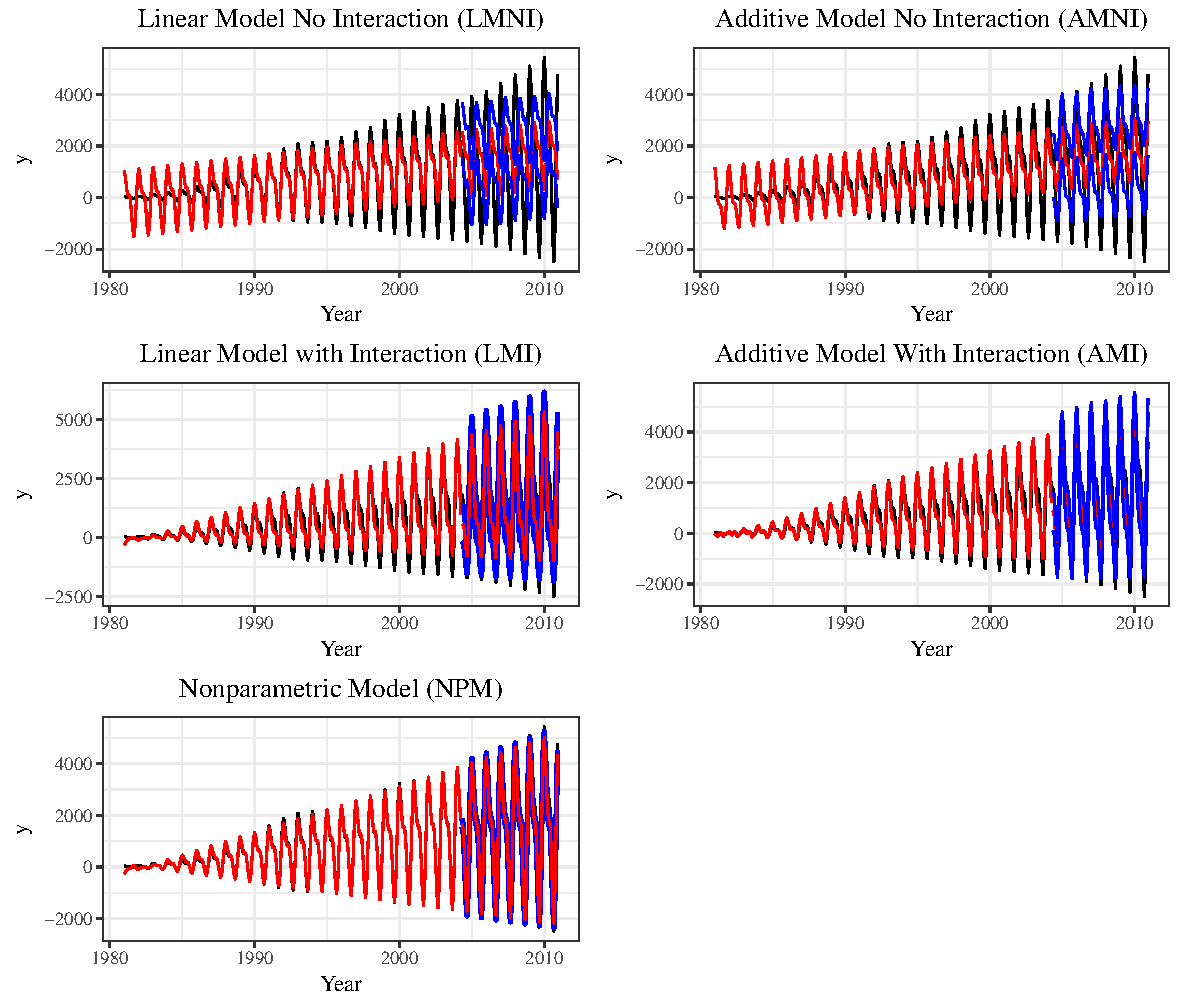
\includegraphics[scale=0.7]{2nd_order_inter.pdf}
\caption{2nd order Fourier series with interaction: fitting and forecasts results for different models.}
\label{fig:2nd Fourier inter}
\end{figure}

\begin{figure}[bp!]
\centering
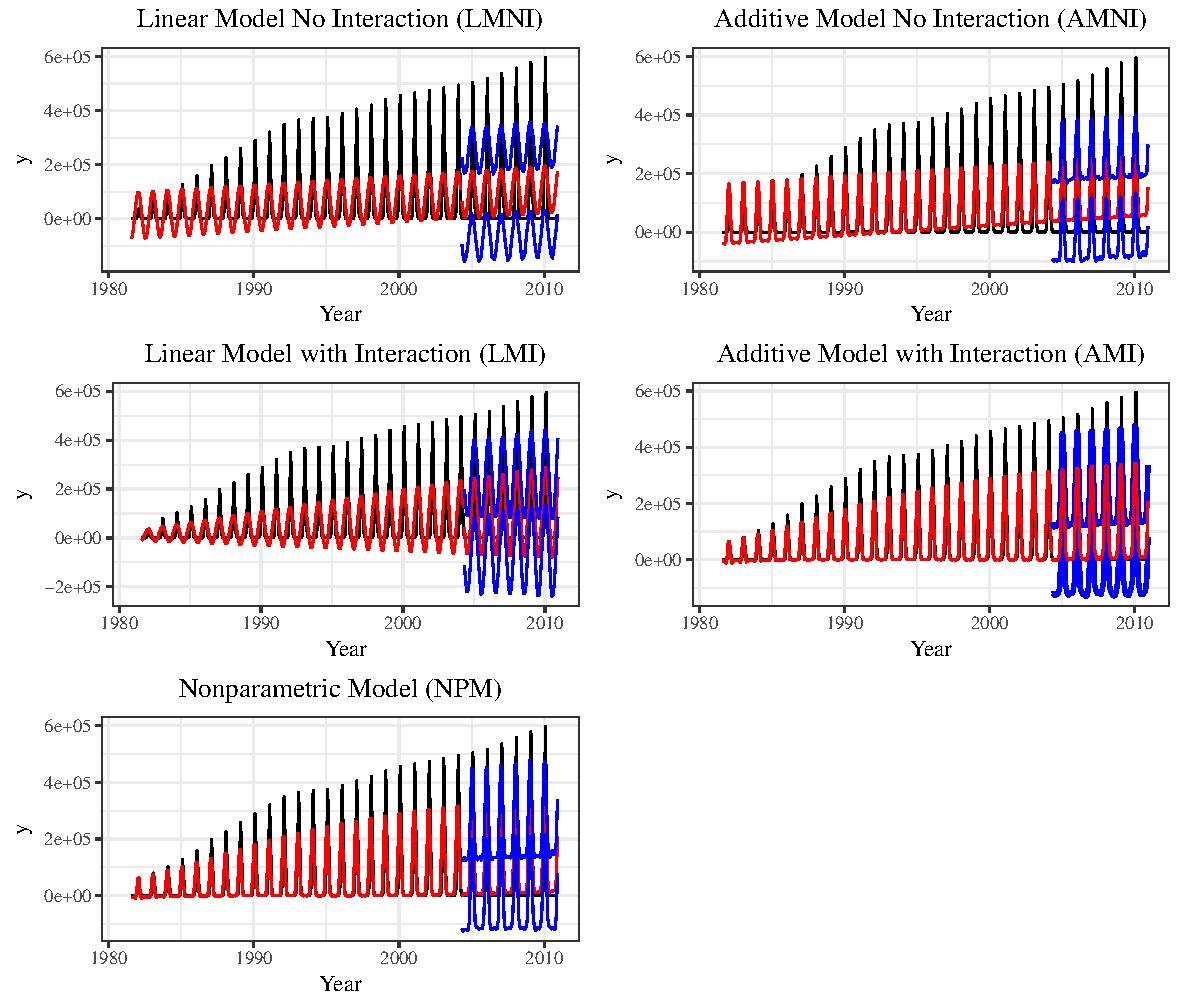
\includegraphics[scale=0.7]{1st_order_complex.pdf}
\caption{1st order Fourier series with non-linear interaction: fitting and forecasts results for different models.}
\label{fig:1st Fourier complex inter}
\end{figure}


\begin{figure}[bp!]
\centering
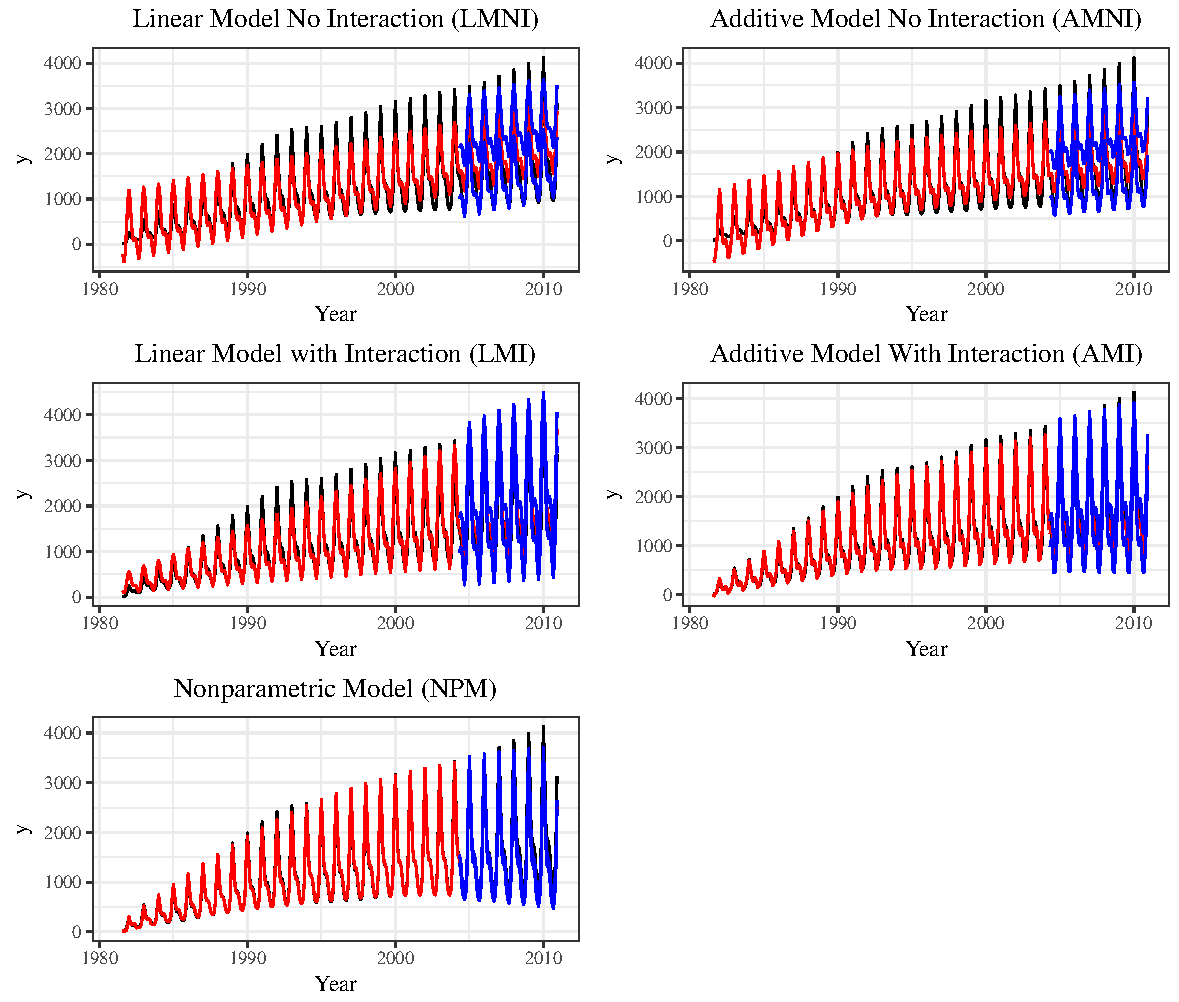
\includegraphics[scale=0.7]{2nd_order_complex.pdf}
\caption{2nd order Fourier series with non-linear interaction: fitting and forecasts results for different models.}
\label{fig:2nd Fourier complex inter}
\end{figure}

\bigskip 



\newpage

\section{Regression Results}\label{Results}

This section reports the results of the Bayesian regressions fitted for the period 1981-2003 both for the time series case (Tables \ref{lmni_ar}, \ref{amni_ar}, \ref{lmi_ar}, \ref{ami_ar} and \ref{npm_ar}), as well as for the longitudinal case (Tables \ref{lmni_age}, \ref{amni_age}, \ref{lmi_age}, \ref{ami_age} and \ref{npm_age}). For the time series case the models include autoregressive errors of order one (AR(1)). The estimates are obtained using 4 Markov chains, each with 4000 iterations, 2000 for warm-up and 2000 for validation, resulting in a total post warm-up sample of 8000 data points. The tables display, from the left to the right column, the potential scale reduction factor ($\hat{R}$), the mean (mean), the standard deviation (sd), the lower $2.5\%$ quantile, the 50\% quantile and the upper $97.5\%$ quantile for all the models. A value of $\hat{R}$ equal to 1 indicates that each chain has stabilized and they are likely to have reached the target distribution\footnote{A $\hat{R}$ significantly bigger than 1 indicates that the between-chain variance is substantially greater than the within-chain variance, warning for the need of a longer simulation.}. 
 
\begin{table}[bp!]
\caption{Linear Model without Interaction (LMNI) with AR(1) errors.}
\label{lmni_ar}
\centering
\begin{tabular}{lrrrrrr}
\\[-1.8ex]\hline 
\hline \\[-1.8ex]
Parameter & $\hat{R}$  & mean & sd & 2.5\% & 50\% & 97.5\% \\ 
\hline \\[-1.8ex] 
Intercept & 1.0 & 8.7 & 0.1 & 8.6 & 8.7 & 8.9 \\ 
trend & 1.0 & 0.4 & 0.2 & 0.0 & 0.4 & 0.7 \\ 
$\sin_{1} + \cos_{1}$ & 1.0 & 0.0 & 0.0 & -0.0 & 0.0 & 0.1 \\ 
$\sin_{2} + \cos_{2}$ & 1.0 & -0.0 & 0.0 & -0.1 & -0.0 & 0.0 \\ 
$\alpha$ & 1.0 & 0.5 & 0.1 & 0.4 & 0.5 & 0.6 \\ 
  \hline \\[-1.8ex] 
$\sigma_{\epsilon}$  & 1.0 & 0.3 & 0.0 & 0.2 & 0.3 & 0.3 \\ 
\\[-1.8ex]\hline 
\hline \\[-1.8ex] 
\end{tabular}
\end{table}

\begin{table}[bp!]
\caption{Additive Model without Interaction (AMNI) with AR(1) errors.}
\label{amni_ar}
\centering
\begin{tabular}{lrrrrrr}
\\[-1.8ex]\hline 
\hline \\[-1.8ex] 
Parameter & $\hat{R}$  & mean & sd & 2.5\% & 50\% & 97.5\% \\ 
\hline \\[-1.8ex] 
Intercept & 1.0 & 8.8 & 0.0 & 8.8 & 8.8 & 8.9 \\ 
$\alpha$ & 1.0 & 0.2 & 0.1 & 0.1 & 0.2 & 0.4 \\ 
\hline \\[-1.8ex] 
$\sigma_{\lambda_{\text{trend}}}$ & 1.0 & 2.7 & 0.8 & 1.5 & 2.5 & 4.7 \\ 
$\sigma_{\lambda_{\sin_{1}+\cos_{1}}}$ & 1.0 & 1.4 & 0.7 & 0.5 & 1.2 & 3.2 \\ 
$\sigma_{\lambda_{\sin_{2}+\cos_{2}}}$ & 1.0 & 1.0 & 0.7 & 0.3 & 0.8 & 2.8 \\ 
$\sigma_{\epsilon}$                    & 1.0 & 0.2 & 0.0 & 0.2 & 0.2 & 0.2 \\ 
\\[-1.8ex]\hline 
\hline \\[-1.8ex] 
\end{tabular}
\end{table}



In order to fully characterize the two semiparametric models, we add to the parametric values of the splines' coefficients a portray of the smooth terms, see Figure (\ref{fig:smooth gam}).
\begin{figure}[bp!]
\begin{minipage}{.33\linewidth}
\centering
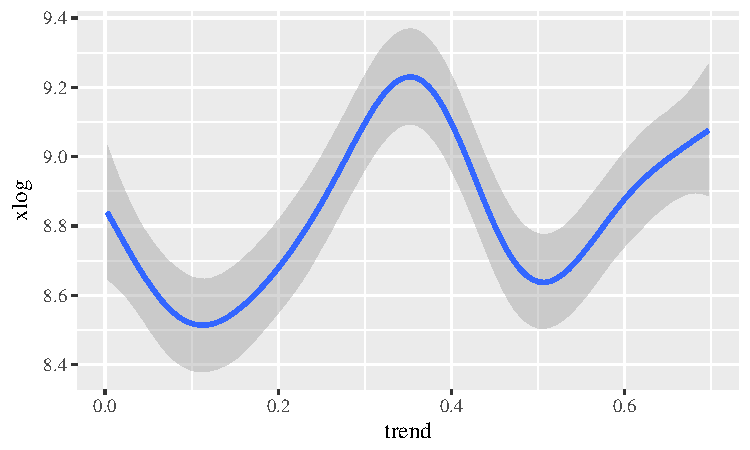
\includegraphics[width=\columnwidth, height=4cm]{smooth1_b_gamm_2004.pdf}
\end{minipage}
\begin{minipage}{.33\linewidth}
\centering
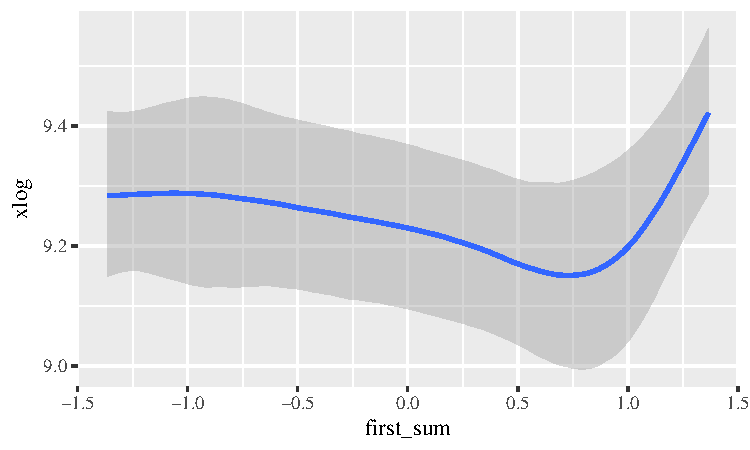
\includegraphics[width=\columnwidth, height=4cm]{smooth2_b_gamm_2004.pdf}
\end{minipage}
\begin{minipage}{.33\linewidth}
\centering
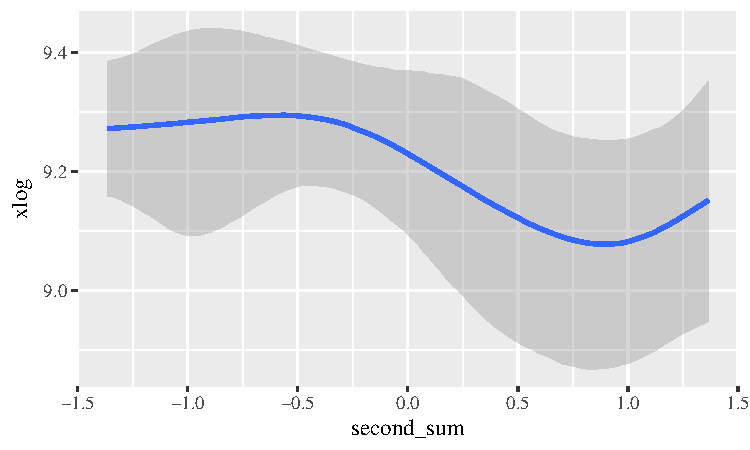
\includegraphics[width=\columnwidth, height=4cm]{smooth3_b_gamm_2004.pdf}
\end{minipage}
\vskip 0.5cm
\caption{Visualization of the non-linear functions of the additive model without interaction (AMNI). The left plot shows the monthly trend, the center plot $(\sin_{1} + \cos_{1})$ and the right plot $(\sin_{2} + \cos_{2})$. The central blue lines are the mean values of the dependent variable immigration (xlog) as a function of the x axis (trend, first sum=$(\sin_{1} + \cos_{1})$, second sum=$(\sin_{2} + \cos_{2})$. The dark grey bands depict the standard errors of the estimates and represent the credible intervals.}
\label{fig:smooth gam}
\end{figure}


\begin{table}[bp!]
\caption{Linear Model with Interaction (LMI) with AR(1) errors.}
\label{lmi_ar}
\centering
\begin{tabular}{lrrrrrr}
\\[-1.8ex]\hline 
\hline \\[-1.8ex] 
Parameter & $\hat{R}$  & mean & sd & 2.5\% & 50\% & 97.5\% \\ 
\hline \\[-1.8ex] 
Intercept & 1.0 & 8.7 & 0.1 & 8.6 & 8.7 & 8.8 \\ 
trend & 1.0 & 0.4 & 0.2 & 0.1 & 0.4 & 0.7 \\ 
$\sin_{1} + \cos_{1}$ & 1.0 & 0.1 & 0.0 & -0.0 & 0.1 & 0.2 \\ 
$\sin_{2} + \cos_{2}$ & 1.0 & -0.0 & 0.0 & -0.1 & -0.0 & 0.1 \\ 
$(\sin_{1} + \cos_{1})$*trend & 1.0 & -0.2 & 0.1 & -0.5 & -0.2 & 0.0 \\ 
$(\sin_{2} + \cos_{2})$*trend  & 1.0 & -0.1 & 0.1 & -0.2 & -0.1 & 0.1 \\ 
$\alpha$ & 1.0 & 0.5 & 0.1 & 0.4 & 0.5 & 0.6 \\ 
  \hline \\[-1.8ex] 
$\sigma_{\epsilon}$ & 1.0 & 0.3 & 0.0 & 0.2 & 0.3 & 0.3 \\ 
\\[-1.8ex]\hline 
\hline \\[-1.8ex] 
\end{tabular}
\end{table}


\begin{table}[bp!]
\caption{Additive Model with Interaction (AMI) with AR(1) errors.}
\label{ami_ar}
\centering
\begin{tabular}{lrrrrrr}
\\[-1.8ex]\hline 
\hline \\[-1.8ex] 
Parameter & $\hat{R}$  & mean & sd & 2.5\% & 50\% & 97.5\% \\ 
\hline \\[-1.8ex] 
Intercept & 1.0 & 8.8 & 0.0 & 8.8 & 8.8 & 8.9 \\ 
$\alpha$ & 1.0 & 0.2 & 0.1 & 0.1 & 0.2 & 0.4 \\ 
\hline \\[-1.8ex] 
$\sigma_{\lambda_{\text{trend}}}$ & 1.0 & 2.7 & 0.8 & 1.5 & 2.5 & 4.6 \\ 
$\sigma_{\lambda_{\sin_{1}+\cos_{1}}}$  & 1.0 & 0.9 & 0.8 & 0.0 & 0.8 & 2.8 \\ 
$\sigma_{\lambda_{\sin_{2}+\cos_{2}}}$  & 1.0 & 0.8 & 0.7 & 0.0 & 0.6 & 2.5 \\ 
$\sigma_{\lambda_{\text{trend} \sin_{1}+\cos_{1}}}$  & 1.0 & 0.2 & 0.1 & 0.0 & 0.2 & 0.5 \\ 
$\sigma_{\lambda_{\text{trend} \sin_{2}+\cos_{2}}}$  & 1.0 & 0.1 & 0.1 & 0.0 & 0.1 & 0.4 \\ 
$\sigma_{\epsilon}$ & 1.0 & 0.2 & 0.0 & 0.2 & 0.2 & 0.2 \\ 

\\[-1.8ex]\hline 
\hline \\[-1.8ex] 
\end{tabular}
\end{table}


\begin{table}[bp!]
\caption{Nonparametric Model (NPM) with AR(1) errors.}
\label{npm_ar}
\centering
\begin{tabular}{lrrrrrr}
\\[-1.8ex]\hline 
\hline \\[-1.8ex] 
Parameter & $\hat{R}$  & mean & sd & 2.5\% & 50\% & 97.5\% \\ 
\hline \\[-1.8ex] 
Intercept & 1.0 & 8.9 & 0.0 & 8.8 & 8.9 & 8.9 \\ 
$\alpha$ & 1.0 & 0.6 & 0.0 & 0.5 & 0.6 & 0.7 \\ 
$\sigma_{\lambda_{\text{trend}, \sin_{1}+\cos_{1}, \sin_{2}+\cos_{2}}}$ & 1.0 & 0.1 & 0.0 & 0.1 & 0.1 & 0.2 \\ 
$\sigma_{\epsilon}$  & 1.0 & 0.2 & 0.0 & 0.2 & 0.2 & 0.2 \\ 
\\[-1.8ex]\hline 
\hline \\[-1.8ex] 
\end{tabular}
\end{table}




\begin{table}[bp!]
\caption{Linear Model without Interaction (LMNI) by Age.}
\label{lmni_age}
\centering
\begin{tabular}{lrrrrrr}
\\[-1.8ex]\hline 
\hline \\[-1.8ex]
Parameter & $\hat{R}$  & mean & sd & 2.5\% & 50\% & 97.5\% \\ 
\hline \\[-1.8ex] 
Intercept & 1.0 & 5.8 & 0.0 & 5.7 & 5.8 & 5.8 \\ 
trend & 1.0 & 0.3 & 0.0 & 0.3 & 0.3 & 0.4 \\
$\sin_{1} + \cos_{1}$ & 1.0 & 0.0 & 0.0 & -0.0 & 0.0 & 0.0 \\ 
$\sin_{2} + \cos_{2}$ & 1.0 & -0.0 & 0.0 & -0.0 & -0.0 & 0.0 \\ 
Age & 1.0 & -0.1 & 0.0 & -0.1 & -0.1 & -0.1 \\ 
  \hline \\[-1.8ex] 
$\sigma_{\epsilon}$  & 1.0 & 0.9 & 0.0 & 0.9 & 0.9 & 0.9 \\ 
\\[-1.8ex]\hline 
\hline \\[-1.8ex] 
\end{tabular}
\end{table}


\begin{table}[bp!]
\caption{Additive Model without Interaction (AMNI) by Age.}
\label{amni_age}
\centering
\begin{tabular}{lrrrrrr}
\\[-1.8ex]\hline 
\hline \\[-1.8ex] 
Parameter & $\hat{R}$  & mean & sd & 2.5\% & 50\% & 97.5\% \\ 
\hline \\[-1.8ex] 
Intercept & 1.0 & 3.4 & 0.0 & 3.4 & 3.4 & 3.4 \\ 
\hline \\[-1.8ex] 
$\sigma_{\lambda_{\text{trend}}}$       & 1.0 & 3.2 & 0.9 & 2.0 & 3.0 & 5.5 \\
$\sigma_{\lambda_{\sin_{1}+\cos_{1}}}$  & 1.0 & 0.1 & 0.1 & 0.0 & 0.0 & 0.2 \\ 
$\sigma_{\lambda_{\sin_{2}+\cos_{2}}}$  & 1.0 & 0.1 & 0.1 & 0.0 & 0.0 & 0.2 \\
$\sigma_{\epsilon}$                    & 1.0 & 0.5 & 0.0 & 0.5 & 0.5 & 0.5 \\
$\sigma_{\lambda_{Age}}$                & 1.0 & 4.4 & 2.0 & 2.2 & 3.9 & 9.5 \\  
\\[-1.8ex]\hline 
\hline \\[-1.8ex] 
\end{tabular}
\end{table}

  
\begin{table}[bp!]
\caption{Linear Model with Interaction (LMI) by Age.}
\label{lmi_age}
\centering
\begin{tabular}{lrrrrrr}
\\[-1.8ex]\hline 
\hline \\[-1.8ex] 
Parameter & $\hat{R}$  & mean & sd & 2.5\% & 50\% & 97.5\% \\ 
\hline \\[-1.8ex] 
Intercept & 1.0 & 5.8 & 0.0 & 5.7 & 5.8 & 5.8 \\ 
trend & 1.0 & 0.3 & 0.0 & 0.3 & 0.3 & 0.4 \\ 
$\sin_{1} + \cos_{1}$ & 1.0 & -0.0 & 0.0 & -0.0 & -0.0 & 0.0 \\ 
$\sin_{2} + \cos_{2}$ & 1.0 & -0.0 & 0.0 & -0.0 & -0.0 & 0.0 \\ 
$(\sin_{1} + \cos_{1})$*trend & 1.0 & 0.0 & 0.0 & -0.0 & 0.0 & 0.1 \\ 
$(\sin_{2} + \cos_{2})$*trend & 1.0 & 0.0 & 0.0 & -0.0 & 0.0 & 0.1 \\ 
Age & 1.0 & -0.1 & 0.0 & -0.1 & -0.1 & -0.1 \\ 
  \hline \\[-1.8ex] 
$\sigma_{\epsilon}$  & 1.0 & 0.9 & 0.0 & 0.9 & 0.9 & 0.9 \\
\\[-1.8ex]\hline 
\hline \\[-1.8ex] 
\end{tabular}
\end{table}

\begin{table}[!htbp]
\caption{Additive Model with Interaction (AMI) by Age.}
\label{ami_age}
\centering
\begin{tabular}{lrrrrrr}
\\[-1.8ex]\hline 
\hline \\[-1.8ex] 
Parameter & $\hat{R}$  & mean & sd & 2.5\% & 50\% & 97.5\% \\ 
\hline \\[-1.8ex] 
Intercept & 1.0 & 3.4 & 0.0 & 3.4 & 3.4 & 3.4 \\ 
\hline \\[-1.8ex] 
$\sigma_{\lambda_{\text{trend}}}$    & 1.0  & 3.5 & 1.0 & 2.1 & 3.3 & 5.8 \\  
$\sigma_{\lambda_{\sin_{1}+\cos_{1}}}$ & 1.0 & 0.1 & 0.1 & 0.0 & 0.1 & 0.3 \\  
$\sigma_{\lambda_{\sin_{2}+\cos_{2}}}$  & 1.1 & 0.1 & 0.1 & 0.0 & 0.0 & 0.5 \\ 
$\sigma_{\lambda_{\text{trend} \sin_{1}+\cos_{1}}}$  & 1.0 & 0.0 & 0.0 & 0.0 & 0.0 & 0.0 \\  
$\sigma_{\lambda_{\text{trend} \sin_{2}+\cos_{2}}}$  & 1.0 & 0.0 & 0.0 & 0.0 & 0.0 & 0.0 \\  
$\sigma_{\lambda_{Age}}$ & 1.0 & 5.3 & 1.3 & 3.5 & 5.0 & 8.5 \\ 
$\sigma_{\epsilon}$                   & 1.0 & 0.5 & 0.0 & 0.5 & 0.5 & 0.5 \\  
\\[-1.8ex]\hline 
\hline \\[-1.8ex] 
\end{tabular}
\end{table}


\begin{table}[!htbp]
\caption{Nonparametric Model (NPM) by Age.}
\label{npm_age}
\centering
\begin{tabular}{lrrrrrr}
\\[-1.8ex]\hline 
\hline \\[-1.8ex] 
Parameter & $\hat{R}$  & mean & sd & 2.5\% & 50\% & 97.5\% \\ 
\hline \\[-1.8ex] 
Intercept & 1.0 & 3.4 & 0.0 & 3.4 & 3.4 & 3.4 \\ 
\hline \\[-1.8ex] 
$\sigma_{\lambda_{\text{trend}, \sin_{1}+\cos_{1}, \sin_{2}+\cos_{2}, Age}}$   & 1.0 & 10.2 & 0.7 & 8.9 & 10.2 & 11.7 \\ 
$\sigma_{\epsilon}$  & 1.0 & 0.5 & 0.0 & 0.4 & 0.5 & 0.5 \\ 
\\[-1.8ex]\hline 
\hline \\[-1.8ex] 
\end{tabular}
\end{table}

\newpage

\section{Diagnostics} \label{subsec:Diagnostics}

The validation of a model is centered around the analysis of its residuals, i.e. the distance between observed and the fitted values. For each regression, we show four diagnostic plots. The first is a comparison between the standardized residuals and the fitted values (top-left). The second is a histogram of the standardized residuals (top-right). The third is a probability-probability plot (PP) which checks how close are the cumulative distribution functions obtained using the data set of the model (bottom-left). The last graph is a comparison of the fitted and the observed values (bottom-right). 

\begin{figure}[bp!]
\centering
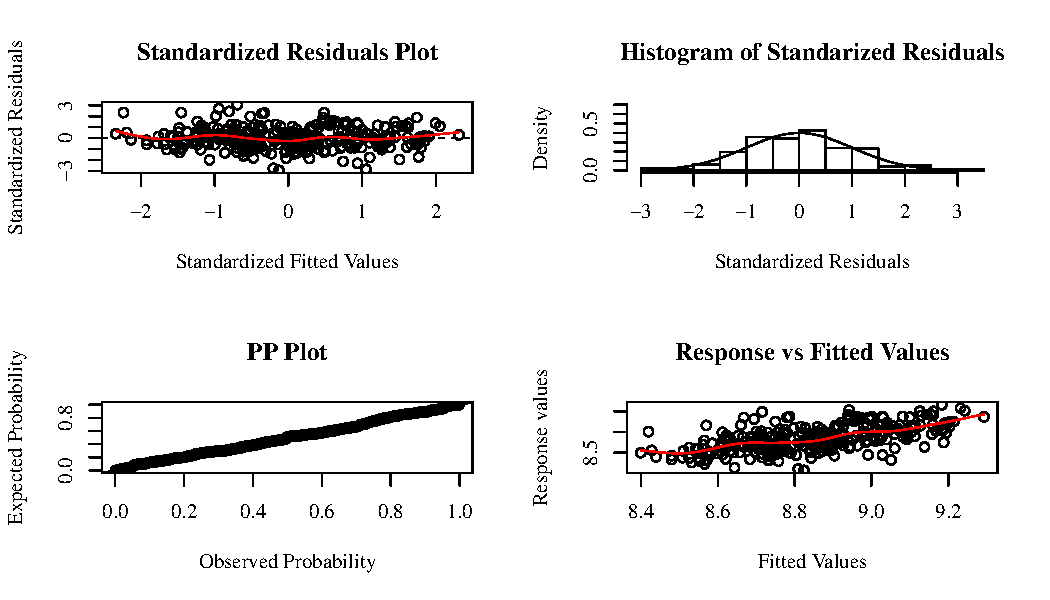
\includegraphics[scale=0.8]{Diag_b_lm_no_2004.pdf}
\caption{Diagnostic Plot Linear Model without Interaction (LMNI).}
\label{fig:Diag LMNI}
\end{figure}

\begin{figure}[bp!]
\centering
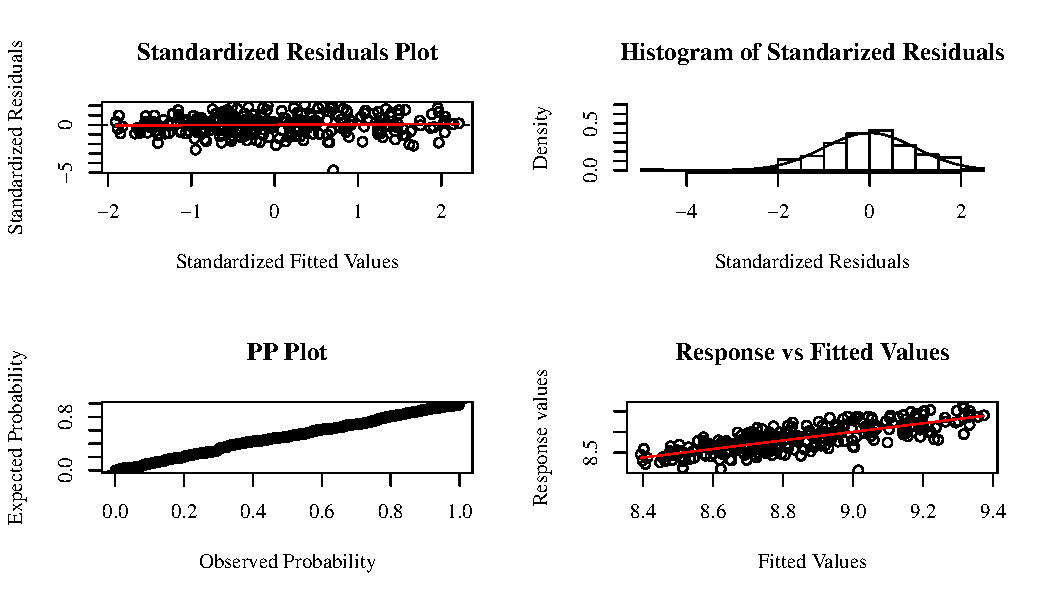
\includegraphics[scale=0.8]{Diag_b_gamm_2004.pdf}
\caption{Diagnostic Plot Additive Model without Interaction (AMNI).}
\label{fig:Diag AMNI}
\end{figure}

\begin{figure}[bp!]
\centering
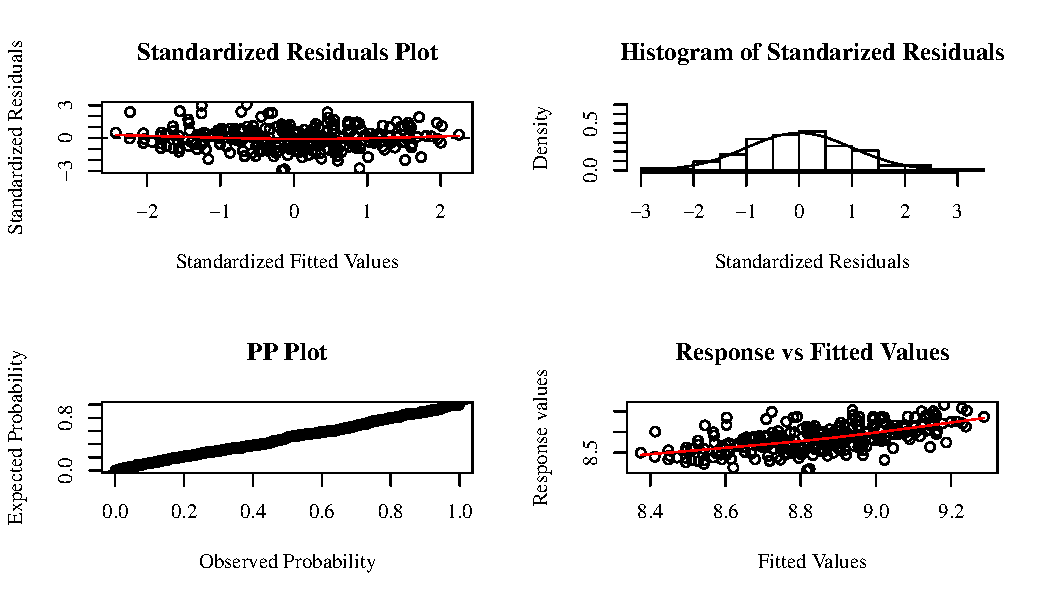
\includegraphics[scale=0.8]{Diag_b_lm_2004.pdf}
\caption{Diagnostic Plot Linear Model with Interaction (LMI).}
\label{fig:Diag LMI}
\end{figure}

\begin{figure}[bp!]
\centering
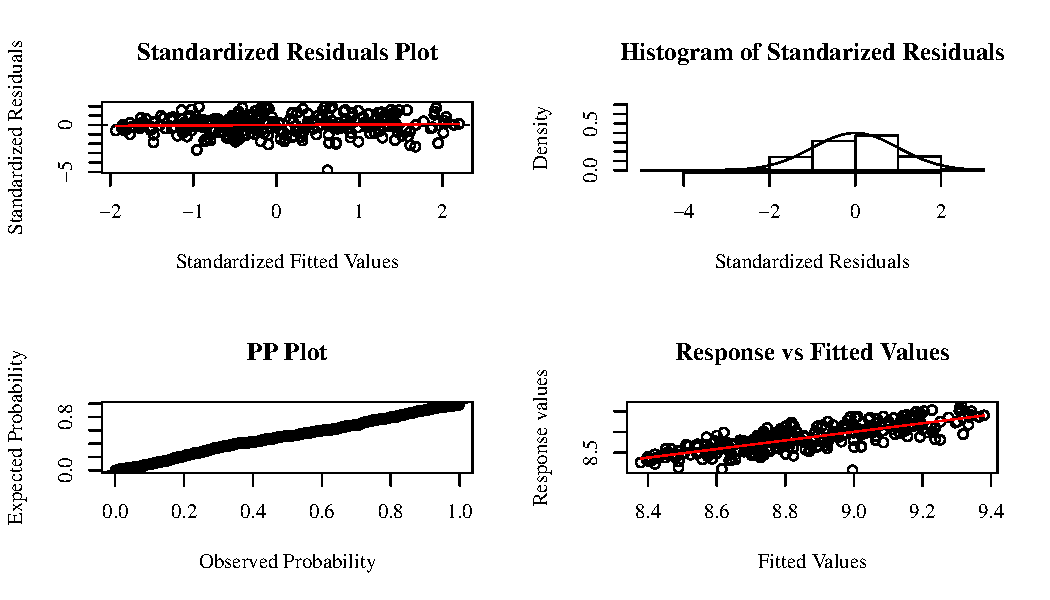
\includegraphics[scale=0.8]{Diag_b_gam_comp_2004.pdf}
\caption{Diagnostic Plot Additive Model with Interaction (AMI).}
\label{fig:Diag AMI}
\end{figure}

\begin{figure}[bp!]
\centering
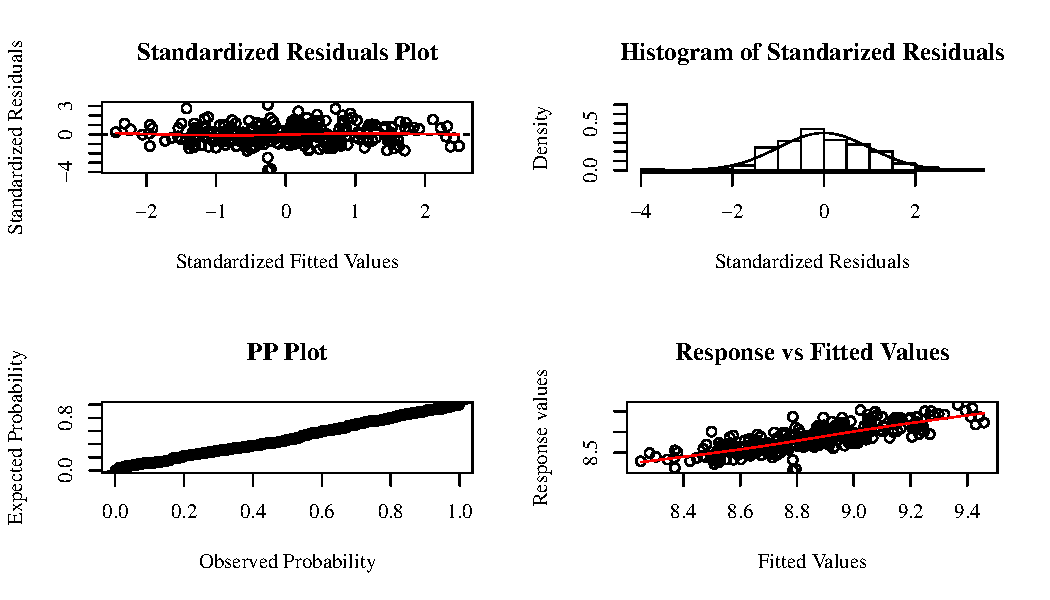
\includegraphics[scale=0.8]{Diag_b_vc_2004.pdf}
\caption{Diagnostic Plot Nonparametric Model with Interaction (NPM).}
\label{fig:Diag NPM}
\end{figure}

All the models show standardized residuals which are rather random and do not form particular clusters. This regular behaviour is replicated by the histograms of the residuals which are all centered around zero and rather regular in their decline to extreme values. The PP plots show a cumulative distribution function of the model very close to the one of the data generating process (i.e. the fitted values are on the 45 degree line). The same is true for response versus fitted values, which are almost on the bissectrice of the first quadrant.  \\
The results obtained using the disaggregate models are similar to the ones achieved using the aggregate specifications. 

\begin{figure}[bp!]
\centering
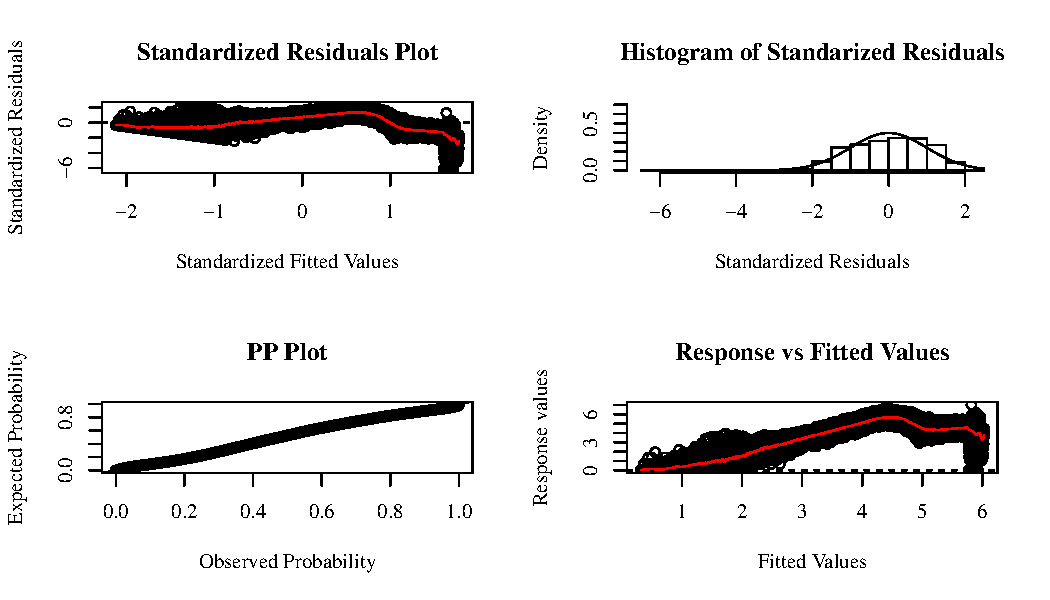
\includegraphics[scale=0.8]{Diag_b_lm_no_age_2004.pdf}
\caption{Diagnostic Plot Linear Model without Interaction (LMNI) by Age.}
\label{fig:Diag LMNI Age}
\end{figure}

\begin{figure}[bp!]
\centering
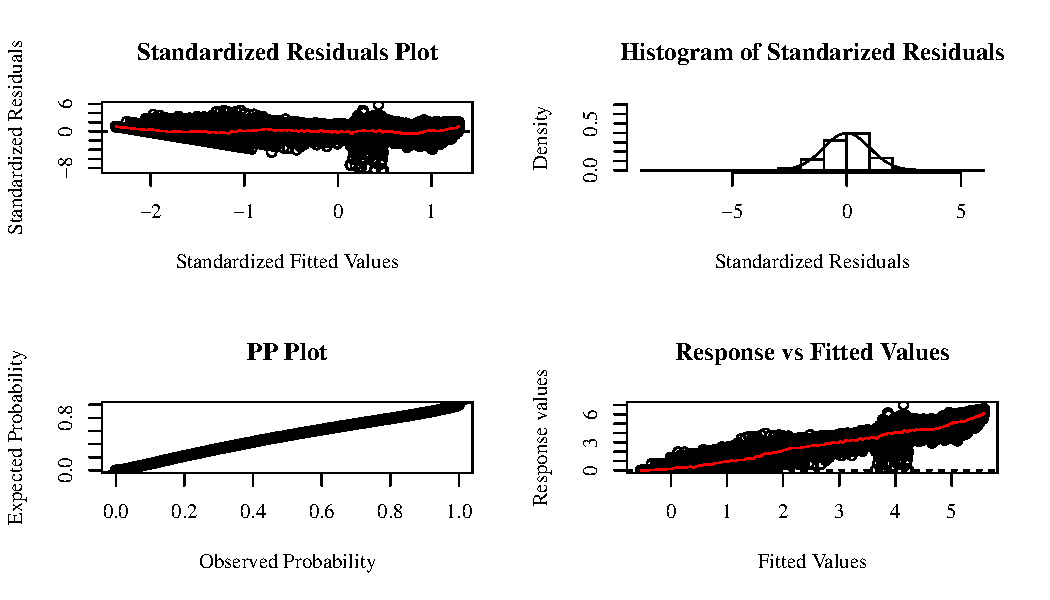
\includegraphics[scale=0.8]{Diag_b_gamm_age_2004.pdf}
\caption{Diagnostic Plot Additive Model without Interaction (AMNI) by Age.}
\label{fig:Diag AMNI Age}
\end{figure}

\begin{figure}[bp!]
\centering
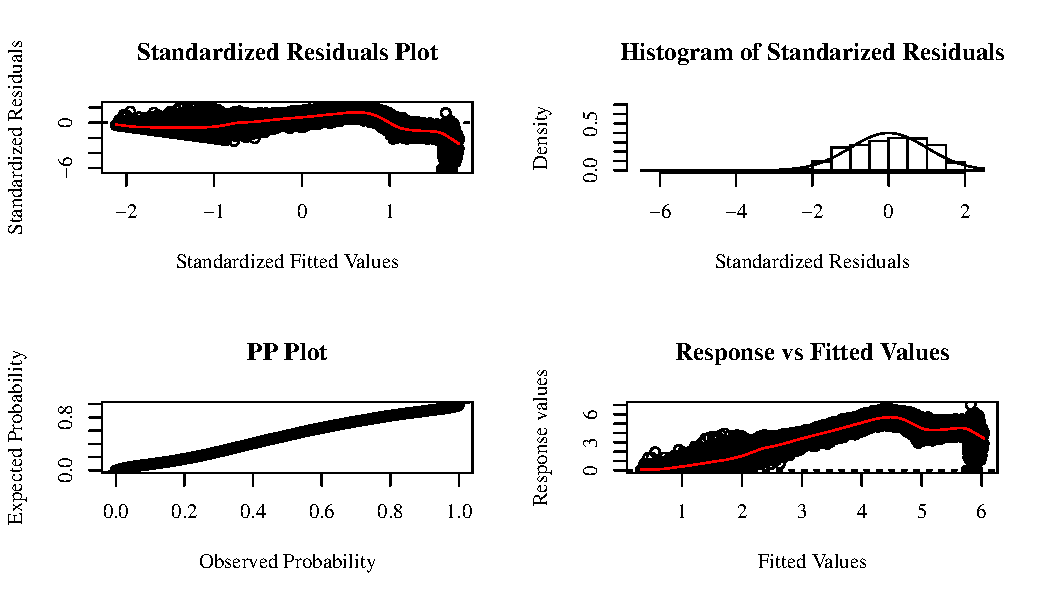
\includegraphics[scale=0.8]{Diag_b_lm_age_2004.pdf}
\caption{Diagnostic Plot Linear Model with Interaction (LMI) by Age.}
\label{fig:Diag LMI Age}
\end{figure}

\begin{figure}[bp!]
\centering
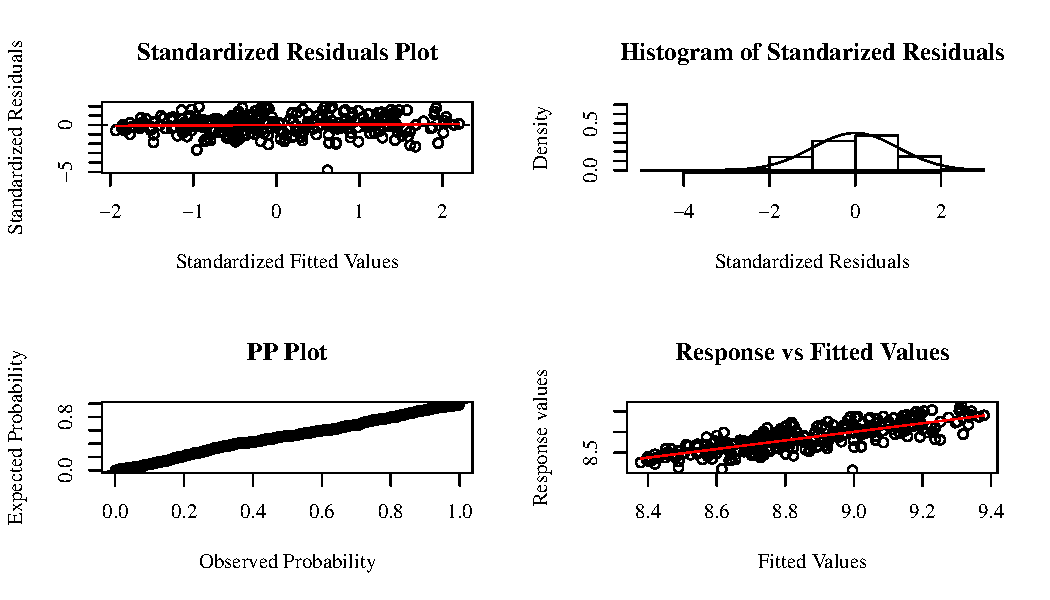
\includegraphics[scale=0.8]{Diag_b_gam_comp_2004.pdf}
\caption{Diagnostic Plot Additive Model with Interaction (AMI) by Age.}
\label{fig:Diag AMI Age}
\end{figure}

\begin{figure}[h!]
\centering
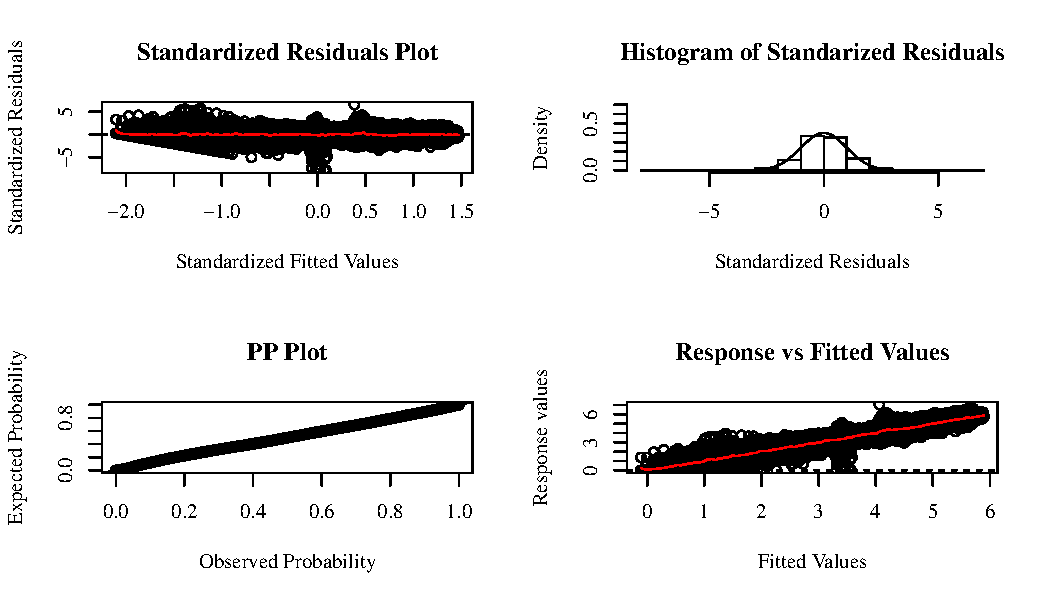
\includegraphics[scale=0.8]{Diag_b_vc_age_2004.pdf}
\caption{Diagnostic Plot Nonparametric Model with Interaction (NPM) by Age.}
\label{fig:Diag NPM Age}
\end{figure}


\newpage

\bibliography{Add_Ref}

\end{document}

